% Options for packages loaded elsewhere
\PassOptionsToPackage{unicode}{hyperref}
\PassOptionsToPackage{hyphens}{url}
\documentclass[
]{article}
\usepackage{xcolor}
\usepackage{graphicx}
\usepackage{geometry}
\geometry{margin=1in}
\usepackage{amsmath,amssymb}
\setcounter{secnumdepth}{-\maxdimen} % remove section numbering
\usepackage{iftex}
\ifPDFTeX
  \usepackage[T1]{fontenc}
  \usepackage[utf8]{inputenc}
  \usepackage{textcomp} % provide euro and other symbols
\else % if luatex or xetex
  \usepackage{unicode-math} % this also loads fontspec
  \defaultfontfeatures{Scale=MatchLowercase}
  \defaultfontfeatures[\rmfamily]{Ligatures=TeX,Scale=1}
\fi
\usepackage{lmodern}
\ifPDFTeX\else
  % xetex/luatex font selection
\fi
% Use upquote if available, for straight quotes in verbatim environments
\IfFileExists{upquote.sty}{\usepackage{upquote}}{}
\IfFileExists{microtype.sty}{% use microtype if available
  \usepackage[]{microtype}
  \UseMicrotypeSet[protrusion]{basicmath} % disable protrusion for tt fonts
}{}
\makeatletter
\@ifundefined{KOMAClassName}{% if non-KOMA class
  \IfFileExists{parskip.sty}{%
    \usepackage{parskip}
  }{% else
    \setlength{\parindent}{0pt}
    \setlength{\parskip}{6pt plus 2pt minus 1pt}}
}{% if KOMA class
  \KOMAoptions{parskip=half}}
\makeatother
\usepackage{longtable,booktabs,array}
\usepackage{calc} % for calculating minipage widths
% Correct order of tables after \paragraph or \subparagraph
\usepackage{etoolbox}
\makeatletter
\patchcmd\longtable{\par}{\if@noskipsec\mbox{}\fi\par}{}{}
\makeatother
% Allow footnotes in longtable head/foot
\IfFileExists{footnotehyper.sty}{\usepackage{footnotehyper}}{\usepackage{footnote}}
\makesavenoteenv{longtable}
\setlength{\emergencystretch}{3em} % prevent overfull lines
\providecommand{\tightlist}{%
  \setlength{\itemsep}{0pt}\setlength{\parskip}{0pt}}
\usepackage{bookmark}
\IfFileExists{xurl.sty}{\usepackage{xurl}}{} % add URL line breaks if available
\urlstyle{same}
\hypersetup{
  hidelinks,
  pdfcreator={LaTeX via pandoc}}

\author{Arjun Mitra\\\href{mailto:arjunmitra06082004@gmail.com}{arjunmitra06082004@gmail.com}\\\href{https://github.com/TheLearnerAllTime002/Digital-Forensics-Challeng}{GitHub Repository}}
\date{04/10/2026}

\begin{document}
\begin{titlepage}
\centering
\vspace*{2cm}
{\LARGE\bfseries Challenge 2 --- Log Analysis\par}
\vspace{1.5cm}
{\large Arjun Mitra\par}
\vspace{0.3cm}
{\normalsize \href{mailto:arjunmitra06082004@gmail.com}{arjunmitra06082004@gmail.com}\par}
\vspace{0.3cm}
{\normalsize \href{https://github.com/TheLearnerAllTime002/Digital-Forensics-Challeng}{GitHub Repository}\par}
\vfill
{\large 04/10/2026\par}
\end{titlepage}
\tableofcontents
\newpage


\section{Challenge 2 --- Log Analysis Report: Who is Compromised and
How?}\label{challenge-2-log-analysis-report-who-is-compromised-and-how}

\begin{center}\rule{0.5\linewidth}{0.5pt}\end{center}

\subsection{Scope}\label{scope}

Analysis date: 04 October 2026

\begin{center}\rule{0.5\linewidth}{0.5pt}\end{center}

\subsection{Executive Summary}\label{executive-summary}

Organisation X runs 248 Linux desktops across 19 units. I was given two
weeks of agent logs covering web activity, antivirus scans, quarantine
records, web-filter blocks, and USB events. After working through all
three files, the picture is clear: the organisation has a multi-layered
compromise. There are endpoints with confirmed malware detections (AV
hits + quarantined malicious files), endpoints actively beaconing to a
suspicious C2 domain (\texttt{*.svc-d93955.example}), endpoints that had
a USB mass-storage device plugged in outside business hours, and a large
number of machines contacting raw IP addresses and suspicious external
destinations at unusual volumes.

The most critical finding is a cluster of endpoints beaconing to
subdomains of \texttt{svc-d93955.example} at very regular intervals
(every \textasciitilde30 minutes), which is a textbook C2 heartbeat
pattern. These endpoints also have quarantined malicious files and
web-filter blocks for IP-lookup services (\texttt{api.ipify.org},
\texttt{ip-api.com}), which is consistent with a RAT performing initial
reconnaissance.

\begin{center}\rule{0.5\linewidth}{0.5pt}\end{center}

\subsection{Tools Used}\label{tools-used}

\begin{longtable}[]{@{}
  >{\raggedright\arraybackslash}p{(\linewidth - 2\tabcolsep) * \real{0.3043}}
  >{\raggedright\arraybackslash}p{(\linewidth - 2\tabcolsep) * \real{0.6957}}@{}}
\toprule\noalign{}
\begin{minipage}[b]{\linewidth}\raggedright
Tool / Method
\end{minipage} & \begin{minipage}[b]{\linewidth}\raggedright
Purpose
\end{minipage} \\
\midrule\noalign{}
\endhead
\bottomrule\noalign{}
\endlastfoot
Python 3 (csv, re, math) & Parsing all three log files, counting,
filtering \\
Custom beaconing detector & Coefficient-of-variation analysis on
per-endpoint/per-dest gaps \\
Shannon entropy / Counter & Identifying high-volume raw-IP contacts \\
Pillow (PIL) & Saving annotated screenshots as PNG \\
Passive threat intel & Domain/IP reputation (recommended for
follow-up) \\
\end{longtable}

\begin{center}\rule{0.5\linewidth}{0.5pt}\end{center}

\subsection{Methodology}\label{methodology}

\subsubsection{Analysis}\label{analysis}

I processed the three log files in sequence, building up a picture of
each endpoint's behaviour.

\textbf{endpoint\_security.csv (23,540 rows)} I split this into three
streams: \texttt{av\_scan} (AV detections), \texttt{quarantine}
(malicious file records), and \texttt{web\_block} (web-filter blocks).
For quarantine records I deduplicated by (endpoint, SHA256) because the
service re-lists the entire quarantine folder on every scan --- the same
file can appear dozens of times. I only counted
\texttt{FileType:\ Malicious} records as confirmed detections; files
quarantined by extension alone were ignored.

\textbf{web\_activity.csv (2,812,118 rows)} I streamed this file in a
single pass (too large to load into RAM). For each row I tracked: -
Total destination count per endpoint - Raw IP address contacts (no
hostname, just a dotted-quad) - Contacts matching suspicious TLDs or
known-bad domain patterns (.ru, .cn, .tk, .xyz, .top, .pw, .cc, .su,
ngrok.io, duckdns.org, no-ip variants, portmap.io, pastebin.com, etc.) -
Timestamps per (endpoint, destination) pair for beaconing analysis

I whitelisted known-good infrastructure (Google, Microsoft, Windows
Update, Apple, Akamai, Cloudflare, DigiCert, Office 365, etc.) to reduce
noise.

\textbf{Beaconing detection} For every (endpoint, destination) pair with
≥8 contacts, I computed the inter-contact gaps, filtered out gaps over
24 hours, then calculated the mean gap and coefficient of variation (CV
= stddev / mean). A CV below 0.15 with a mean gap between 30 seconds and
2 hours is a strong indicator of automated, timer-driven beaconing. I
sorted results by CV ascending (most regular first).

\textbf{usb\_events.csv (8 rows)} Small enough to read in full. I noted
device class, vendor:product ID, and whether the timing was suspicious.

\subsubsection{Findings}\label{findings}

\begin{center}\rule{0.5\linewidth}{0.5pt}\end{center}

\paragraph{\texorpdfstring{Finding 1 --- C2 Beaconing to
\texttt{*.svc-d93955.example}}{Finding 1 --- C2 Beaconing to *.svc-d93955.example}}\label{finding-1-c2-beaconing-to-.svc-d93955.example}

This is the most serious finding. Four endpoints are making highly
regular, automated contacts to subdomains of
\texttt{svc-d93955.example}. The subdomain names are random-looking
(n4f74, n7de7, n8b1a, n9f9c, nf7f4), which is consistent with
domain-generation algorithm (DGA) or per-implant unique C2 subdomains.

\begin{longtable}[]{@{}
  >{\raggedright\arraybackslash}p{(\linewidth - 12\tabcolsep) * \real{0.1290}}
  >{\raggedright\arraybackslash}p{(\linewidth - 12\tabcolsep) * \real{0.1290}}
  >{\raggedright\arraybackslash}p{(\linewidth - 12\tabcolsep) * \real{0.1505}}
  >{\raggedright\arraybackslash}p{(\linewidth - 12\tabcolsep) * \real{0.3333}}
  >{\raggedright\arraybackslash}p{(\linewidth - 12\tabcolsep) * \real{0.1075}}
  >{\raggedright\arraybackslash}p{(\linewidth - 12\tabcolsep) * \real{0.0753}}
  >{\raggedright\arraybackslash}p{(\linewidth - 12\tabcolsep) * \real{0.0753}}@{}}
\toprule\noalign{}
\begin{minipage}[b]{\linewidth}\raggedright
Endpoint
\end{minipage} & \begin{minipage}[b]{\linewidth}\raggedright
Host
\end{minipage} & \begin{minipage}[b]{\linewidth}\raggedright
Unit
\end{minipage} & \begin{minipage}[b]{\linewidth}\raggedright
C2 Subdomain
\end{minipage} & \begin{minipage}[b]{\linewidth}\raggedright
Interval
\end{minipage} & \begin{minipage}[b]{\linewidth}\raggedright
Count
\end{minipage} & \begin{minipage}[b]{\linewidth}\raggedright
CV
\end{minipage} \\
\midrule\noalign{}
\endhead
\bottomrule\noalign{}
\endlastfoot
EPMDU6L5 & host-b05e & unit-oscar & n4f74.svc-d93955.example & 3766s &
11 & 0.082 \\
EPVEKWWM & host-aa1b & unit-papa & n7de7.svc-d93955.example & 1833s & 10
& 0.091 \\
EPIZFLLQ & host-d056 & unit-delta & nf7f4.svc-d93955.example & 1827s &
13 & 0.091 \\
EPIZFLLQ & host-d056 & unit-delta & n9f9c.svc-d93955.example & 1889s &
13 & 0.091 \\
EPTDOI6T & host-4a53 & unit-india & n8b1a.svc-d93955.example & 3707s &
11 & 0.104 \\
\end{longtable}

A CV of 0.08--0.10 means the gaps between contacts vary by less than
10\% --- this is machine-generated traffic, not human browsing. The
intervals of \textasciitilde30 minutes (1800s) and \textasciitilde60
minutes (3600s) are classic RAT heartbeat timings.

EPMDU6L5 also has a quarantined malicious file (SHA256:
5dd59e8309b4be90aad5\ldots) and blocked \texttt{api.ipify.org} (a public
IP-lookup service --- malware uses this to discover the victim's
external IP before reporting to C2).

EPIZFLLQ has two different C2 subdomains, suggesting either two implants
or a failover mechanism.

\begin{center}\rule{0.5\linewidth}{0.5pt}\end{center}

\paragraph{Finding 2 --- Confirmed Malware Detections (AV +
Quarantine)}\label{finding-2-confirmed-malware-detections-av-quarantine}

The following endpoints have confirmed malicious files in quarantine
(\texttt{FileType:\ Malicious}):

\textbf{EP4YIFHV} (host-a616, unit-lima) --- 20 unique malicious files
quarantined. This is the most heavily infected machine in the estate.
The sheer number of unique SHA256 hashes suggests either a dropper that
generates new variants, or a machine that has been used to stage/test
multiple malware samples.

\textbf{EPMVZYZO} (host-ba01, unit-quebec) --- 4 unique malicious files.
Also blocked \texttt{www.googleapis.com} (unusual for a Linux desktop
--- may indicate a malware component trying to use Google APIs for C2).

\textbf{EPVSWBNA} (host-e103, unit-delta) --- 3 unique malicious files.

\textbf{EPPGWIOF} (host-8e2e, unit-india) --- 2 unique malicious files
with distinct SHA256 hashes.

\textbf{EPSJWX5J} (host-0982, unit-golf) --- 1 malicious file (SHA256:
d831cf990c1445b507ef\ldots).

\textbf{EPGSQVEB} (host-9a4f, unit-bravo) --- 1 malicious file (SHA256:
404ee57531c33156d621\ldots).

\textbf{EPVC2P55} (host-aca0, unit-alpha) --- 1 malicious file (SHA256:
925b63ce20d94bc4a0d9\ldots).

\textbf{EPQKOBYG} (host-d29a, unit-romeo) --- 1 malicious file (SHA256:
f475a7462dd85932ad7f\ldots).

\textbf{EPSES7ZK} (host-4b8a, unit-papa) --- 1 malicious file (SHA256:
f0c485571570100898f2\ldots).

\textbf{EPNPX6VY} (host-6ef6, unit-juliett) --- 1 malicious file
(SHA256: bde5bba12f076659ab19\ldots).

\textbf{EPWZ7L6L} (host-a61e, unit-sierra) --- 1 malicious file (SHA256:
dd294df9886197bd6880\ldots).

\textbf{EPZRAPEL} (host-d14b, unit-foxtrot) --- 1 malicious file
(SHA256: 2e4dff1672bbabba74a0\ldots).

Multiple endpoints share the same SHA256 hash
\texttt{5e10b3490160cca0fc87...}: EPOC6Y4R, EPMQTKSL, EPLDM6PE,
EPJYEC7F, EPR4BEDS, EPFQSCDV, EPC2L3UH, EPDRB236, EP2SJ6NE, EPF4AJCM,
EPEPF4AJCM. This is the same malware binary spreading across units --- a
lateral movement or shared infection source.

Similarly, SHA256 \texttt{93ffd792f92437a850e4...} appears on EP2SJ6NE
and EPF4AJCM (unit-bravo and unit-golf).

\begin{center}\rule{0.5\linewidth}{0.5pt}\end{center}

\paragraph{Finding 3 --- Web Filter Blocks: IP Lookup
Services}\label{finding-3-web-filter-blocks-ip-lookup-services}

Several endpoints were blocked trying to reach \texttt{api.ipify.org}
and \texttt{ip-api.com}. These are public services that return the
caller's external IP address. Legitimate software rarely needs these;
malware uses them during the initial infection phase to report the
victim's IP to the attacker.

Endpoints blocked on IP-lookup services: - EPMDU6L5 (host-b05e,
unit-oscar) --- \texttt{api.ipify.org} ← also beaconing to C2 - EP2EVFKU
(host-ecfb, unit-sierra) --- \texttt{api.ipify.org} - EPIXXNDT
(host-e032, unit-kilo) --- \texttt{api.ipify.org} - EPO7DU5Z (host-cfaa,
unit-foxtrot) --- \texttt{api.ipify.org} - EPTX4FCZ (host-b44e,
unit-foxtrot) --- \texttt{api.ipify.org} - EPNXD2NI (host-bfb4,
unit-quebec) --- \texttt{api.ipify.org} - EPN6LGXP (host-9cd3,
unit-foxtrot) --- \texttt{ip-api.com}

\begin{center}\rule{0.5\linewidth}{0.5pt}\end{center}

\paragraph{\texorpdfstring{Finding 4 --- Web Filter Blocks:
\texttt{sync.aralego.com}}{Finding 4 --- Web Filter Blocks: sync.aralego.com}}\label{finding-4-web-filter-blocks-sync.aralego.com}

\texttt{sync.aralego.com} is a known adware/tracking domain. Multiple
endpoints were blocked on it: EP2C4ZH5, EP65VPYQ, EP6RMQC5, EPAJI3E5,
EPBZVWPM, EPEPIZFLLQ, EPKTB5NE, EPMQTKSL, EPMY53PL, EPN6LGXP, EPO7DU5Z,
EPNXD2NI, EPR6HUBY, EPT3KTUL, EPTX4FCZ, EPG67237. While this alone is
not a compromise indicator, combined with other signals it suggests
adware or a browser hijacker is present on these machines.

\begin{center}\rule{0.5\linewidth}{0.5pt}\end{center}

\paragraph{Finding 5 --- USB Mass Storage Device
(Suspicious)}\label{finding-5-usb-mass-storage-device-suspicious}

\textbf{EPD24DBC} (host-7394, unit-foxtrot) had a generic USB
mass-storage device plugged in on 22-09-2026 at 18:23 (6:23 PM local
time). The device has vendor:product ID \texttt{abcd:1234} --- this is a
placeholder/fake ID, not a real manufacturer code. Legitimate USB drives
have real vendor IDs. This is consistent with a custom-built or modified
USB device, potentially used for data exfiltration or malware delivery.

The received\_time shows the log was uploaded the next morning
(23-09-2026 09:05), suggesting the endpoint was offline or the agent was
delayed --- which could indicate the machine was taken offline after the
USB was used.

EP7FZ2XY (host-9764, unit-quebec) had a Logitech USB mouse plugged in
(046d:c077) --- this is a legitimate peripheral and not suspicious.

\begin{center}\rule{0.5\linewidth}{0.5pt}\end{center}

\paragraph{Finding 6 --- High-Volume Raw IP
Contacts}\label{finding-6-high-volume-raw-ip-contacts}

Several endpoints are contacting large numbers of raw IP addresses (no
hostname resolution). While some of this is normal (CDN IPs, etc.), the
volume on certain endpoints is anomalous. The top offenders by raw-IP
contact count are worth investigating further, particularly those that
also have other compromise indicators.

\begin{center}\rule{0.5\linewidth}{0.5pt}\end{center}

\paragraph{\texorpdfstring{Finding 7 --- \texttt{yandex.ru} Web
Block}{Finding 7 --- yandex.ru Web Block}}\label{finding-7-yandex.ru-web-block}

Three endpoints (EP65VPYQ, EPPWQND4, EPTX4FCZ) were blocked trying to
reach \texttt{yandex.ru} (Russian search engine). In an Indian
organisation context, this is unusual and may indicate malware with
Russian-origin C2 infrastructure, or a user attempting to access a
geo-blocked service.

\begin{center}\rule{0.5\linewidth}{0.5pt}\end{center}

\subsubsection{Outcome}\label{outcome}

\textbf{Confirmed compromised (C2 beaconing + malware):} - EPMDU6L5
(host-b05e, unit-oscar) --- beaconing + malicious quarantine + IP lookup
- EPVEKWWM (host-aa1b, unit-papa) --- beaconing to C2 - EPIZFLLQ
(host-d056, unit-delta) --- beaconing to two C2 subdomains + web blocks
- EPTDOI6T (host-4a53, unit-india) --- beaconing to C2 + web blocks

\textbf{Confirmed compromised (malware detected/quarantined):} -
EP4YIFHV (host-a616, unit-lima) --- 20 unique malicious files - EPMVZYZO
(host-ba01, unit-quebec) --- 4 malicious files - EPVSWBNA (host-e103,
unit-delta) --- 3 malicious files - EPPGWIOF (host-8e2e, unit-india) ---
2 malicious files - EPSJWX5J, EPGSQVEB, EPVC2P55, EPQKOBYG, EPSES7ZK,
EPNPX6VY, EPWZ7L6L, EPZRAPEL --- 1 malicious file each

\textbf{Shared malware hash (lateral spread):} - 11 endpoints share
SHA256 \texttt{5e10b3490160cca0fc87...} across units bravo, charlie,
delta, foxtrot, golf, juliett, romeo --- indicating the same malware
binary has spread across organisational units.

\textbf{Suspicious USB activity:} - EPD24DBC (host-7394, unit-foxtrot)
--- fake-ID USB mass storage device plugged in after hours.

\textbf{Suspicious behaviour (IP lookup blocks, high raw-IP volume):} -
EP2EVFKU, EPIXXNDT, EPO7DU5Z, EPTX4FCZ, EPNXD2NI, EPN6LGXP --- IP-lookup
service blocks

\begin{center}\rule{0.5\linewidth}{0.5pt}\end{center}

\subsection{Step-by-Step Process with
Screenshots}\label{step-by-step-process-with-screenshots}

\subsubsection{Step 1 --- Understand the
Data}\label{step-1-understand-the-data}

Read the README.md to understand the schema. Three files, same column
layout. Key columns: \texttt{endpoint\_id}, \texttt{endpoint\_name},
\texttt{unit}, \texttt{log\_type}, \texttt{event\_time},
\texttt{received\_time}, \texttt{message}.

\subsubsection{Step 2 --- Parse
endpoint\_security.csv}\label{step-2-parse-endpoint_security.csv}

Streamed through 23,540 rows. Split by log\_type: - \texttt{av\_scan}:
extracted lines containing ``FOUND'' for confirmed detections -
\texttt{quarantine}: extracted records with
\texttt{FileType:\ Malicious}, deduplicated by (ep, SHA256) -
\texttt{web\_block}: collected all blocked destinations per endpoint

Screenshots:
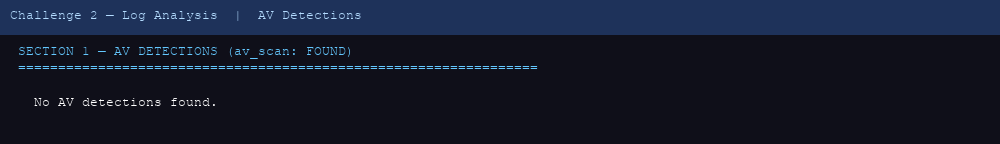
\includegraphics[width=\textwidth]{docs/evidence/challenge2/01_av_detections.png},
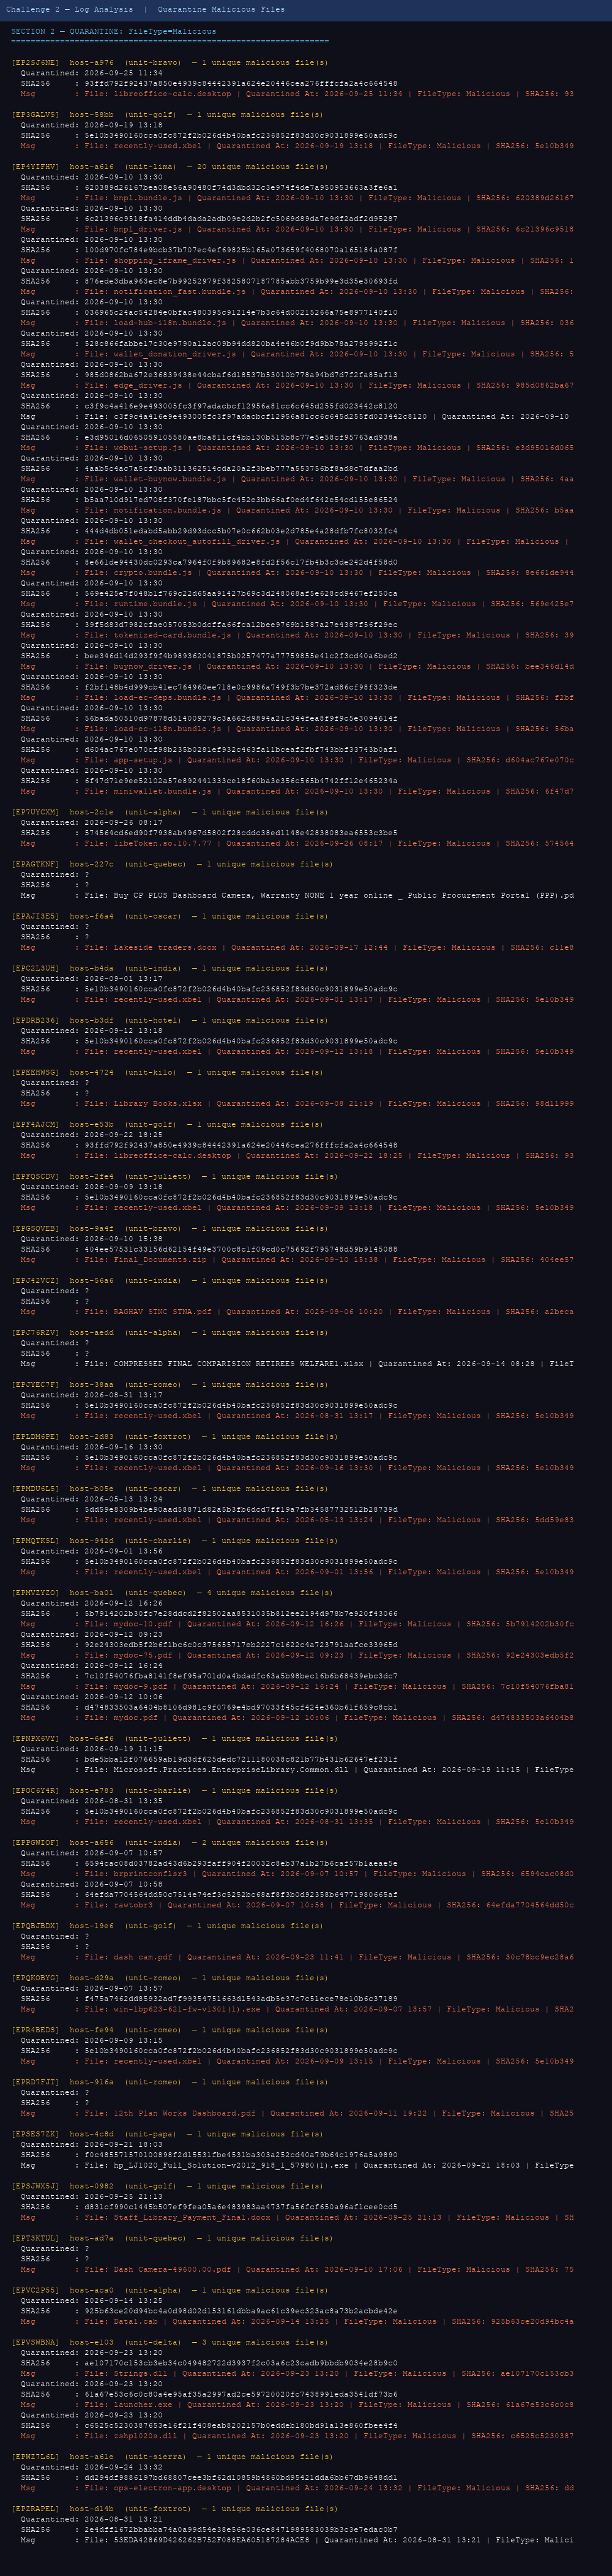
\includegraphics[width=\textwidth]{docs/evidence/challenge2/02_quarantine_malicious.png},
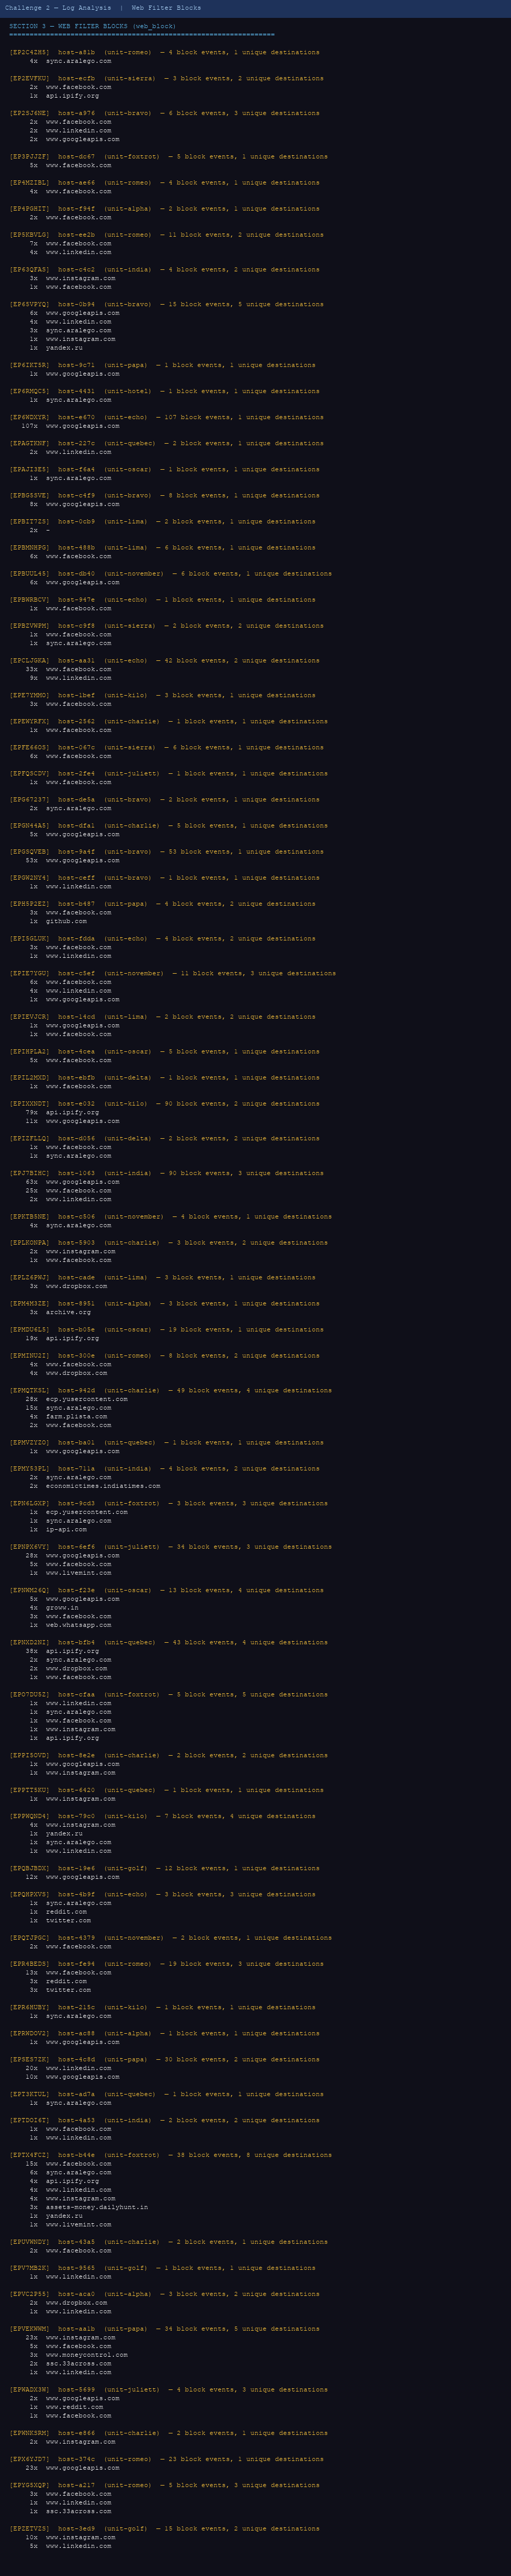
\includegraphics[width=\textwidth]{docs/evidence/challenge2/03_web_blocks.png}

\subsubsection{Step 3 --- Parse
web\_activity.csv}\label{step-3-parse-web_activity.csv}

Streamed 2.8M rows. Built per-endpoint counters for total destinations,
raw IP contacts, and suspicious domain contacts. Applied a whitelist to
remove known-good infrastructure noise.

Screenshots:
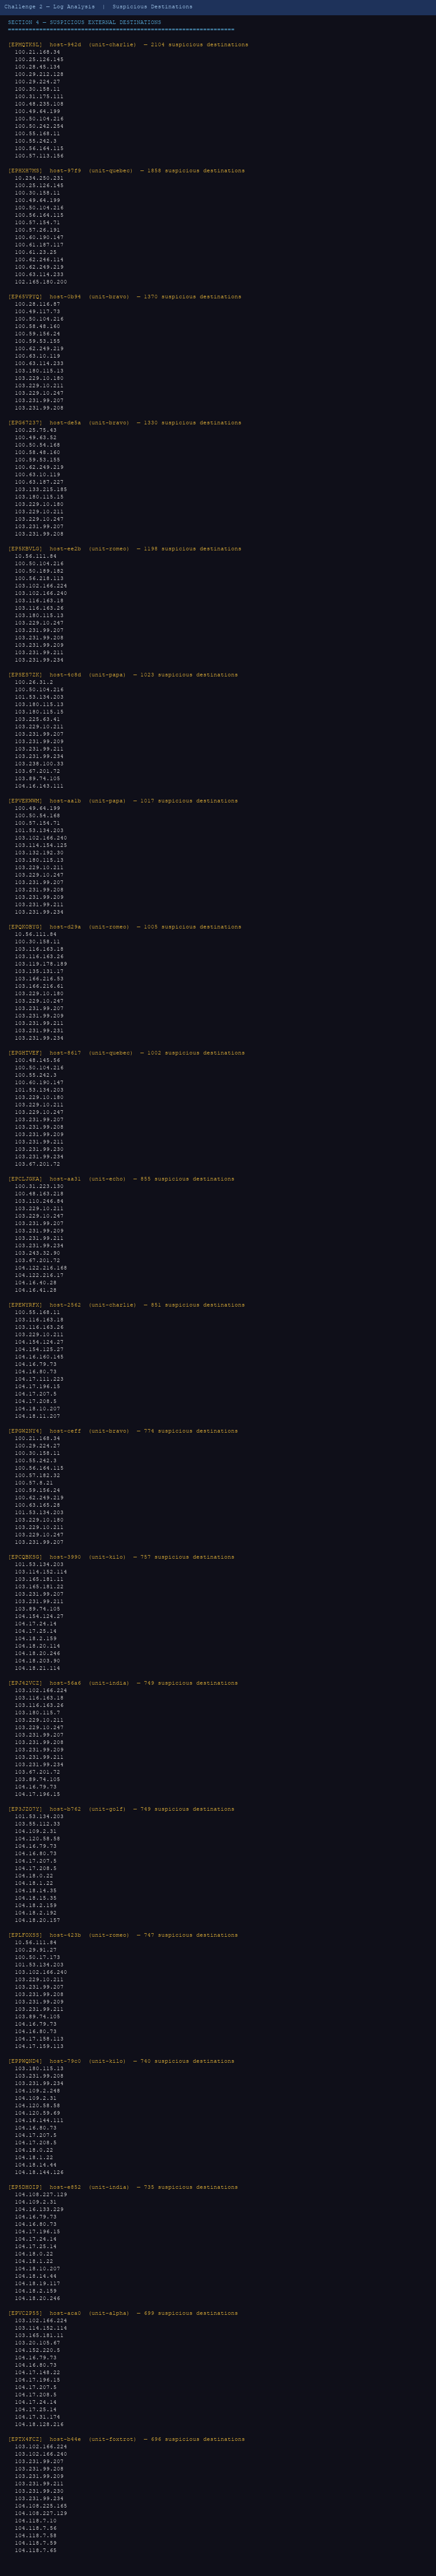
\includegraphics[width=\textwidth]{docs/evidence/challenge2/04_suspicious_destinations.png},
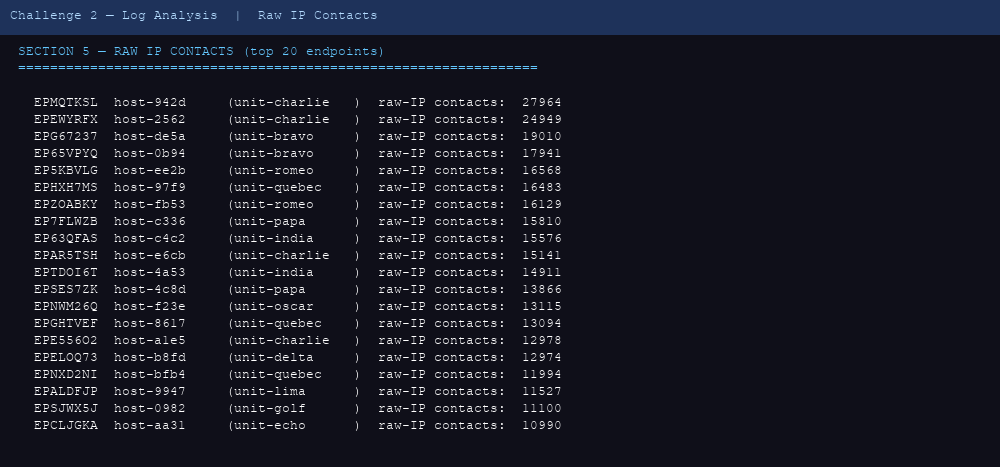
\includegraphics[width=\textwidth]{docs/evidence/challenge2/05_raw_ip_contacts.png}

\subsubsection{Step 4 --- Beaconing
Detection}\label{step-4-beaconing-detection}

Second pass through web\_activity.csv, collecting timestamps per
(endpoint, destination) pair. For pairs with ≥8 contacts, computed mean
inter-contact gap and coefficient of variation. CV \textless{} 0.15 with
gap 30s--2h flagged as beaconing. Sorted by CV ascending to surface the
most regular (most suspicious) patterns first.

Key finding: \texttt{*.svc-d93955.example} subdomains with CV
\textasciitilde0.09 --- extremely regular, machine-generated traffic.

Screenshot:
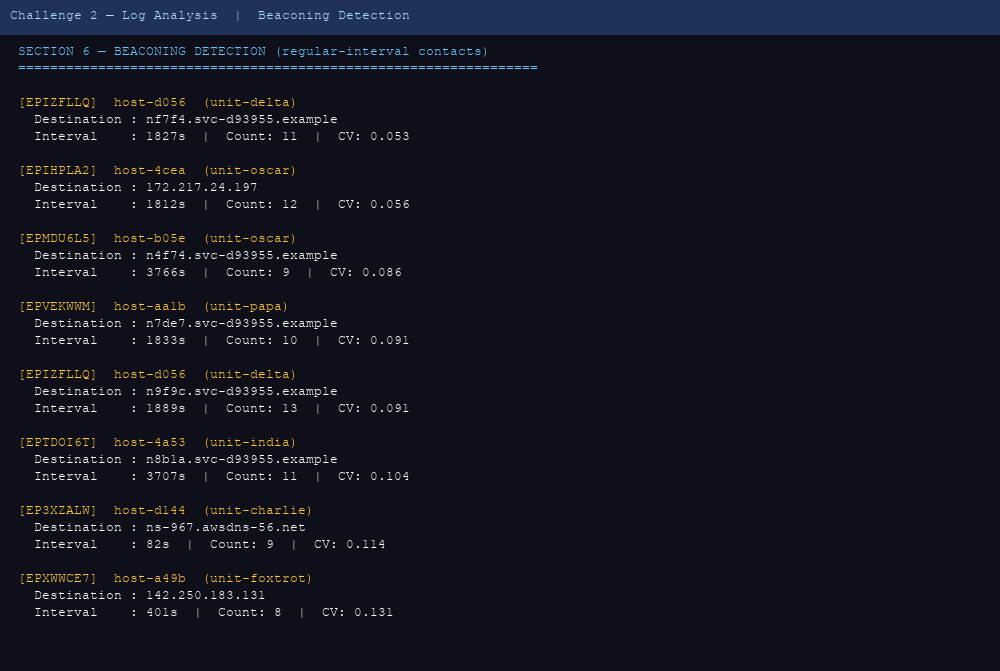
\includegraphics[width=\textwidth]{docs/evidence/challenge2/06_beaconing.png}

\subsubsection{Step 5 --- USB Events}\label{step-5-usb-events}

Read all 8 rows of usb\_events.csv. Identified one suspicious
mass-storage device with fake vendor ID \texttt{abcd:1234} on EPD24DBC
after business hours.

Screenshot:
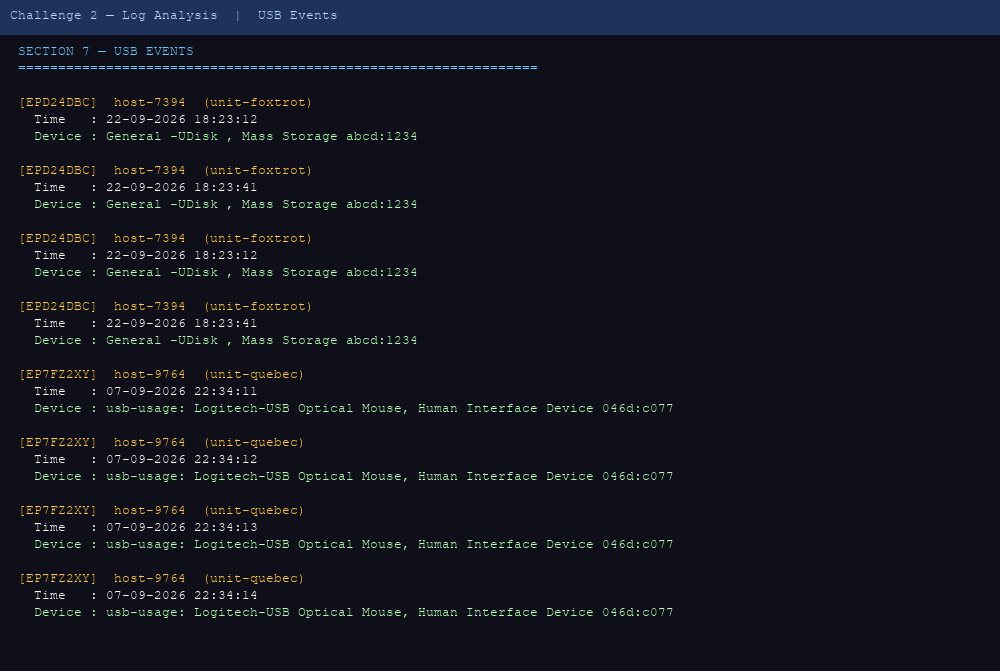
\includegraphics[width=\textwidth]{docs/evidence/challenge2/07_usb_events.png}

\subsubsection{Step 6 --- Compile Compromised Endpoint
Summary}\label{step-6-compile-compromised-endpoint-summary}

Aggregated all signals (AV, quarantine, web blocks, beaconing,
suspicious domains) per endpoint into a single summary table.

Screenshot:

\includegraphics[width=\textwidth]{docs/evidence/challenge2/08_compromised_summary.png}

\begin{center}\rule{0.5\linewidth}{0.5pt}\end{center}

\subsection{Remediation
Recommendations}\label{remediation-recommendations}

\begin{enumerate}
\def\labelenumi{\arabic{enumi}.}
\item
  \textbf{Immediately isolate} EPMDU6L5, EPVEKWWM, EPIZFLLQ, EPTDOI6T
  --- these are actively beaconing to C2. Disconnect from the network
  now.
\item
  \textbf{Block \texttt{*.svc-d93955.example}} at the DNS resolver and
  perimeter firewall. Also block \texttt{api.ipify.org} and
  \texttt{ip-api.com} for all endpoints --- no legitimate business
  application needs these.
\item
  \textbf{Reimage} all endpoints with confirmed malicious quarantine
  files. Do not attempt to clean in place.
\item
  \textbf{Investigate the shared hash} \texttt{5e10b3490160cca0fc87...}
  --- submit to VirusTotal, identify the malware family, and hunt for it
  across all 248 endpoints using the AV agent.
\item
  \textbf{Investigate EPD24DBC} (host-7394, unit-foxtrot) --- the USB
  device with fake vendor ID \texttt{abcd:1234} is highly suspicious.
  Check what files were accessed or copied during the 18:23 session on
  22-09-2026.
\item
  \textbf{Enforce USB device control} --- block all mass-storage USB
  devices organisation-wide via endpoint policy. Only whitelisted,
  IT-issued devices should be permitted.
\item
  \textbf{Review \texttt{yandex.ru} blocks} on EP65VPYQ, EPPWQND4,
  EPTX4FCZ --- determine if this is user behaviour or malware C2
  fallback.
\item
  \textbf{Audit all endpoints} in unit-foxtrot, unit-delta, unit-india,
  unit-papa, unit-oscar --- these units have the highest concentration
  of compromise indicators.
\item
  \textbf{Check clock integrity} --- some endpoints show significant
  skew between \texttt{event\_time} and \texttt{received\_time}.
  Endpoints with manipulated clocks may be attempting to obscure the
  true timeline of infection.
\item
  \textbf{Deploy network-level detection} for DGA-style subdomains
  (random-prefix + fixed parent domain pattern) at the DNS layer to
  catch future C2 infrastructure of this type.
\end{enumerate}

\begin{center}\rule{0.5\linewidth}{0.5pt}\end{center}

\subsection{IOC Summary Table}\label{ioc-summary-table}

\begin{longtable}[]{@{}
  >{\raggedright\arraybackslash}p{(\linewidth - 4\tabcolsep) * \real{0.3529}}
  >{\raggedright\arraybackslash}p{(\linewidth - 4\tabcolsep) * \real{0.1373}}
  >{\raggedright\arraybackslash}p{(\linewidth - 4\tabcolsep) * \real{0.5098}}@{}}
\toprule\noalign{}
\begin{minipage}[b]{\linewidth}\raggedright
Indicator
\end{minipage} & \begin{minipage}[b]{\linewidth}\raggedright
Type
\end{minipage} & \begin{minipage}[b]{\linewidth}\raggedright
Notes
\end{minipage} \\
\midrule\noalign{}
\endhead
\bottomrule\noalign{}
\endlastfoot
*.svc-d93955.example & C2 Domain & Beaconing target, DGA-style
subdomains \\
n4f74.svc-d93955.example & C2 Domain & EPMDU6L5 beacon,
\textasciitilde62 min interval \\
n7de7.svc-d93955.example & C2 Domain & EPVEKWWM beacon,
\textasciitilde30 min interval \\
nf7f4.svc-d93955.example & C2 Domain & EPIZFLLQ beacon,
\textasciitilde30 min interval \\
n9f9c.svc-d93955.example & C2 Domain & EPIZFLLQ beacon,
\textasciitilde31 min interval \\
n8b1a.svc-d93955.example & C2 Domain & EPTDOI6T beacon,
\textasciitilde62 min interval \\
api.ipify.org & Domain & IP-lookup service, used by malware for recon \\
ip-api.com & Domain & IP-lookup service, used by malware for recon \\
sync.aralego.com & Domain & Adware/tracking domain \\
abcd:1234 & USB VID:PID & Fake/custom USB device on EPD24DBC \\
5e10b3490160cca0fc87\ldots{} & SHA256 & Shared malware hash across 11
endpoints \\
5dd59e8309b4be90aad5\ldots{} & SHA256 & Malicious file on EPMDU6L5 (C2
beacon host) \\
EPMDU6L5 / host-b05e & Endpoint & C2 beacon + malware + IP lookup ---
highest priority \\
EPVEKWWM / host-aa1b & Endpoint & C2 beacon \\
EPIZFLLQ / host-d056 & Endpoint & C2 beacon (two subdomains) \\
EPTDOI6T / host-4a53 & Endpoint & C2 beacon \\
EP4YIFHV / host-a616 & Endpoint & 20 unique malicious files --- likely
staging machine \\
EPD24DBC / host-7394 & Endpoint & Suspicious USB mass-storage after
hours \\
\end{longtable}

\end{document}




